\subsection{Second Derivatives}
\begin{definition}
    [Second Derivative]
    refers to the derivative of the derivative of a function. \\
    Give $f(x)$, the second derivative of $f(x)$ is $$f''(x)$$\\
    Given function $y = \cdots$, the second derivative of $y = \cdots$ is 
    $$\frac{d^2y}{dx^2}$$
    Information you can gain from second derivative
    \begin{itemize}
        \item the slopes of the tangents at any '$x$' value of the first derivative graph. 
        \item how 'quickly' these first derivative y values are changing (magnitude) and the trend in these first derivative y values. 
    \end{itemize}
\end{definition}

We will use the function $s(t) = 6t^2 + t^3$ to show you the informations bring by second derivative

\begin{center}
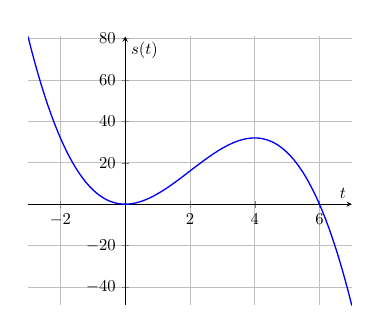
\begin{tikzpicture}[scale = 0.6]
\begin{axis}[
    axis lines = middle,
    xlabel = $t$,
    ylabel = {$s(t)$},
    domain=-3:7,
    samples=100,
    grid=both
]
\addplot[blue, thick] {6*x^2 - x^3};
\end{axis}
\end{tikzpicture}
\end{center}

Here is the first derivative of $s(t)$ $$s'(t) = -3t^2 + 12t$$
\begin{center}
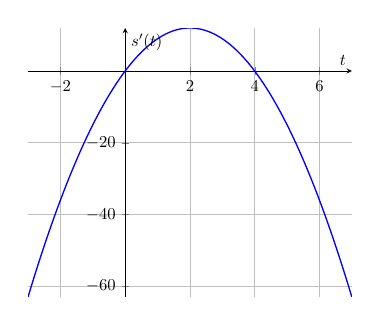
\begin{tikzpicture}[scale = 0.6]
\begin{axis}[
    axis lines = middle,
    xlabel = $t$,
    ylabel = {$s'(t)$},
    domain=-3:7,
    samples=100,
    grid=both
]
\addplot[blue, thick] {12*x - 3*x^2};
\end{axis}
\end{tikzpicture}
\end{center}

Here is the second derivative $$s''(t) = -6t + 12$$
\begin{center}
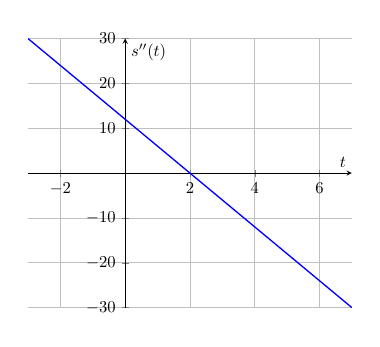
\begin{tikzpicture}[scale = 0.6]
\begin{axis}[
    axis lines = middle,
    xlabel = $t$,
    ylabel = {$s''(t)$},
    domain=-3:7,
    samples=100,
    grid=both
]
\addplot[blue, thick] {-6*x + 12};
\end{axis}
\end{tikzpicture}
\end{center}

Let's explain the relationship between the function $f(x)$, $f'(x)$. \\
\begin{proposition}
    Given function $f(x)$, and its derivative $f'(x)$

    \begin{center}
        As $f'(x)$ moving away from x-axis $\implies$ speeding up in $f(x)$\\
        As $f'(x)$ moving towards x-axis $\implies$ the region in the origin is slowing down. \\
         $\forall x \in \R, f'(x) = 0$ such that $f(x)$ is local minimum/maximum 
    \end{center}
\end{proposition}

Let's connect the $f(x)$ and $f''(x)$
\begin{proposition}
    Given function $f(x)$ and $f''(x)$

    \begin{center}
        $\forall x \in \R, f''(x) > 0$ such that $f(x)$ is concave up on $\R$.\\
        $\forall x \in \R, f''(x) < 0$ such that $f(x)$ is concave down on $\R$.\\
        $\forall x \in \R, f''(x) = 0$ such that $f(x)$ is a inflection point. \\
    \end{center}
\end{proposition}

For $f(x), f'(x)\text{ , and } f''(x)$, we have such identity
$$\forall x \in \R, f(x)f'(x) < 0, s.t. \text{ the original curve is slowing down}$$
$$\forall x \in \R, f(x)f'(x) > 0, s.t. \text{ the original curve is speeding up}$$